\chapter{Robust anomaly diagnosis with calibrating normalizing flows}\label{ch:icml}

The methods developed in previous chapters rely heavily on simulation to predict and repair failures in autonomous systems. Although simulation-driven testing is an important part of the development process for these systems, the ultimate goal is to deploy the system in the real world. Unfortunately, testing a system in the real world presents a number of challenges for the methods presented thus far in this thesis. Whereas simulation testing allows us to vary environmental parameters in order to preemptively predict failures, in reality we are often faced with the problem of analyzing a failure after the fact (often called a \textit{post-mortem} analysis). The goal of this analysis is to infer, based on data collected during a particular failure event, what went wrong; i.e. what changes in the environment were associated with the observed failure.

This analysis is challenging for a number of reasons. First, data collected from a system operating in the real world is often noisy and prone to outliers. Second, if we have been responsible in developing and deploying our system, failures should be relatively rare, meaning that while we may have a large amount of data from normal operation of the system, we typically have very little data from the failure itself. This data imbalance makes it difficult to apply many learning and inference methods directly to post-mortem analysis.

To formalize this problem, we can frame post-mortem analysis as a Bayesian inverse problem (IP), where we aim to infer the distribution of latent variables $z$ from noisy observations $x$ of a stochastic process $x \sim p(x | z; y)$, where $y$ are known context variables~\cite{stuartInverseProblemsBayesian2010,molinaroNeuralInverseOperators2023,liuOptimizationAmortizedInverse2023,asimInvertibleGenerativeModels2020}\footnote{In this chapter, we use $x$, $y$, and $z$ to denote the observation, context, and latent variables to align with standard inverse problem notation. In the context of the notation used in previous chapters, $x$ denotes the system's behavior, represented as a trace of states $s_1, \ldots, s_T$, while $y$ and $z$ denote known and unknown components of the exogenous parameters, respectively}.
%
In a traditional Bayesian IP setting, we are given one or more i.i.d. samples $\set{y_i, x_i}$, but in the anomaly diagnosis setting there is a \textit{data imbalance} between a large number of samples $\Dn = \set{y_i, x_i}_{i=1, \ldots, N_n}$ from nominal operations and a much smaller number of examples observed during the anomaly $\Df = \set{y_j, x_j}_{j=1, \ldots, N_a}$, where $N_a \ll N_n$. This data-constrained setting is related to, but distinct from, out-of-distribution detection (where $\Df$ is not known;~\cite{liangEnhancingReliabilityOutofdistribution2020,hendrycksDeepAnomalyDetection2018,kirichenkoWhyNormalizingFlows2020}) and few-shot learning (where $\Df$ is unknown during training but known at inference time;~\cite{wangGeneralizingFewExamples2020}).

Given these data, anomaly diagnosis aims to infer the \textit{nominal distribution} $p(z | \Dn)$ conditioned solely on the nominal data and the \textit{anomaly distribution} $p(z | \Df, \Dn)$ conditioned on all available data. Sampling from each of these distributions helps us understand what changes in the latent variables were associated with the observed anomaly (helping us ask ``what went wrong''), while comparing the likelihoods of these distributions allows us to test for the presence of anomalies in future data. Unfortunately, imbalanced data in anomaly diagnosis problems makes it challenging to apply existing inference methods, which risk either overfitting to noise in the limited anomaly data or underfitting the anomaly in favor of the large nominal dataset.

In this chapter, we address this gap by introducing \ouralg, or calibrated normalizing flows. To make full use of available data, \ouralg{} amortizes inference over both the nominal and anomaly data, learning a shared representation for both posteriors, but it prevents overfitting using a novel subsample-then-calibrate approach to learn an optimal representation for the anomaly posterior.
%
In contrast to existing methods for regularized distribution learning, our method does not require manual hyperparameter tuning, and it exceeds the performance of hand-tuned baselines on a range of challenging data-constrained inference problems.

To demonstrate the real-world applicability of \ouralg{}, we apply our method to a post-mortem analysis of the 2022 Southwest Airlines scheduling crisis, which stranded more than 2 million passengers during a winter storm and led to more than \$750 million in financial losses~\cite{roseSouthwestWillPay2023}. Our analysis provides new insights into the dynamics of the Southwest network and suggests that an imbalanced distribution of aircraft at key airports (other than those affected by the storm) may have contributed to the failure.

The paper is organized as follows. Section~\ref{ch:icml:background} provides relevant background on inverse problems and normalizing flows. Section~\ref{ch:icml:methodology} introduces \ouralg{}, and Section~\ref{ch:icml:experiments} compares our approach to existing regularized inference methods on a range of benchmarks. Section~\ref{ch:icml:wn-case-study} presents our main case study: a data-driven post-mortem analysis of the 2022 Southwest Airlines scheduling crisis. Section~\ref{ch:icml:conclusion} concludes and identifies directions for future work.

\section{Background}\label{ch:icml:background}

\subsection{Variational inference for Bayesian inverse problems}

There is a large body of work dealing with IPs from a Bayesian perspective. Historically, Markov chain Monte Carlo (MCMC) methods have been the gold standard for posterior sampling, but the computational expense of MCMC motivates the use of approximate algorithms like variational inference (VI;~\cite{stuartInverseProblemsBayesian2010}). These methods optimize the parameters of a variational guide that approximates the true posterior $q_{\phi}(z) \approx p(z | x; y)$ by maximizing the evidence lower bound (ELBO) on the dataset $\mathcal{D}$,
\begin{align}
    \mathcal{L}(\phi, \mathcal{D}) = & \expectation_{(x, y) \in \mathcal{D}} \expectation_{z\sim q_{\phi}(z)}\left[ \log \frac{p(x, z; y)}{q_\phi (z)} \right]. \label{ch:icml:eq:elbo}
\end{align}
In general, $q$ may also depend on $x$ and $y$~\cite{kingmaAutoEncodingVariationalBayes2014}.

\subsection{Normalizing flows}

$\mathcal{L}$ is maximized when the variational guide matches the true posterior $q_\phi(z) = p(z | x; y)$. Classical VI methods use simple representations for $q_\phi$, such as independent Gaussians, which are often not capable of matching the true posterior, motivating the use of more flexible guides like normalizing flows (NFs). NFs represent $q_\phi$ as the transformation of a simple base distribution $q_0$ (e.g. Gaussian) through an invertible mapping; e.g., $z = f_\phi(z_0)$, with $z_0 \sim \mathcal{N}(0, I)$ and a smooth bijection $f_\phi$ with inverse $f_\phi^{-1}$~\cite{tabakDensityEstimationDual2010, rezendeVariationalInferenceNormalizing2015}. We can sample from this distribution by passing samples from the base distribution through $f$, and the exact likelihood is given in terms of the Jacobian of $f$ as:
\begin{equation}
    \log q_\phi(z) = \log q_0(f^{-1}(z)) - \log \abs{\det J_f\pn{f^{-1}(z)}}.
\end{equation}

Normalizing flows have seen substantial success as flexible representations for image generation, density estimation, and inverse problems~\cite{asimInvertibleGenerativeModels2020}. Substantial effort has been devoted to developing flows based on different choices for $f$~\cite{papamakariosNormalizingFlowsProbabilistic2021,grathwohlFFJORDFreeFormContinuous2018,onkenOTFlowFastAccurate2021,huangNeuralAutoregressiveFlows2018,durkanNeuralSplineFlows2019}. Our focus in this chapter is not on proposing and evaluating a new architecture for $f$ but rather on addressing the challenges involved in training normalizing flows in data-constrained settings.

\section{Method: calibrated normalizing flows}\label{ch:icml:methodology}

The key challenge in applying existing VI methods, including those using normalizing flows, to our setting is the imbalance in the size of the nominal and failure datasets. Relying solely on anomaly data risks overfitting to noise in those data, but using both datasets risks underfitting the anomaly in favor of the much larger nominal dataset.

Existing methods attempt to resolve this issue by first learning the nominal posterior, then using it as a prior to regularize the anomaly posterior. This is commonly done by training $q_{\phi_n}$ on nominal data alone, then learning $q_{\phi_a}$ subject to a penalty on divergence from the nominal distribution~\cite{asimInvertibleGenerativeModels2020,higginsBetaVAELearningBasic2016}; for example, by solving:
%
\begin{align}
    \phi_{n} & = \argmax_\phi \mathcal{L}(\phi, \mathcal{D}_n),                                                                                 \\
    \phi_{a} & = \argmax_\phi \mathcal{L}(\phi, \mathcal{D}_a) - \beta D_{KL}(q_{\phi} || q_{\phi_{n}}), \label{ch:icml:eq:elbo_kl_regularized}
\end{align}
where $\beta$ is a hyperparameter that controls how close the anomaly posterior is to the nominal distribution. The Kullback-Leibler divergence $D_{KL}$ is often used to measure closeness to the nominal distribution, but other measures may be used instead. The main challenge with this approach is that $\beta$ can be difficult to tune. As we show in Fig.~\ref{ch:icml:fig:toy_example}, too little regularization results in overfitting to noise in the scarce data, while too much makes it difficult to distinguish between the nominal and anomalous cases. There is no clear choice for how much regularization is appropriate, and so it must be tuned manually, leaving substantial room for error.

\begin{figure}[ht]
    \centering
    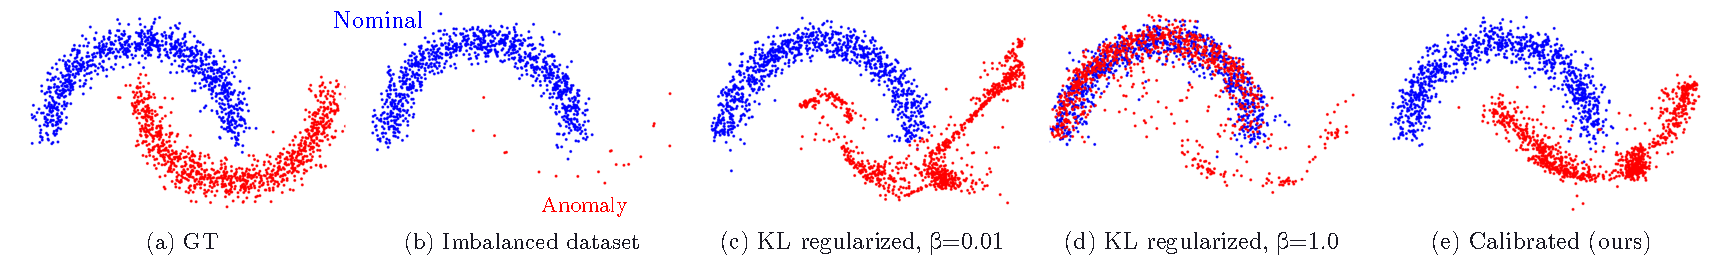
\includegraphics[width=\textwidth]{images/icml/toy_results_overview.pdf}
    \caption{\textbf{Illustrating the effect of data imbalance.} (a) The ground truth distribution. (b) An imbalanced dataset. (c) When the regularization strength $\beta$ is too small, existing methods overfit to noise in the anomaly dataset. (d) When $\beta$ is too large, the learned distribution underfits the anomaly and struggles to distinguish between nominal and anomalous data. (e) Our method yields a more accurate reconstruction of the anomaly distribution by constraining the divergence between the nominal and anomaly distributions.}
    \label{ch:icml:fig:toy_example}
\end{figure}

Our first insight is that instead of choosing a specific regularization strength $\beta$ beforehand, we can train a single normalizing flow to learn a family of distributions that interpolate between the nominal and anomaly distributions (e.g. by training a single normalizing flow with a label to distinguish between the two cases), then choose the best representation from this family of distributions. Unfortunately, it is not immediately clear how the ``best'' representation should be chosen; simply picking the representation that best explains the anomaly data (i.e. by maximizing the evidence for the anomaly data) will just recover the anomaly distribution learned without any regularization. Instead, our second key insight is that we can interpolate between the distribution of the nominal data and the distribution of different random subsets of the anomaly data, then find the best interpolation between these subsets that explains the full anomaly dataset. The family of distributions learned using this approach is shown in Fig.~\ref{ch:icml:fig:grid}, where we use a one-hot label to learn the distribution of each random subset. We see that distributions learned for each of the random subsets is somewhat overfit to noise in that particular subset, but we can find a better representation of the anomaly distribution by finding the label that interpolates between these distributions and maximizes the evidence on the overall anomaly dataset. This approach takes inspiration from the intuition behind robust regression methods like RANSAC~\cite{fischlerRandomSampleConsensus1981}.

\begin{figure}[ht]
    \centering
    \includegraphics[width=\textwidth]{images/icml/grid.png}
    \caption{\textbf{Uncalibrated vs. calibrated posteriors.} (Left) The family of distributions learned prior to the calibration step. The red and blue points are samples from the nominal $q_\phi(z; \mathbf{0})$ and anomaly posteriors $q_\phi(z; \lambda \mathbf{1}_i)$ for $\lambda \in [0, 1]$, respectively. Even though the individual posteriors overfit to their respective subsets, the calibrated posterior (right) fits well across the full anomaly dataset.}
    \label{ch:icml:fig:grid}
\end{figure}

We call this approach calibrated normalizing flows, or \ouralg{}. The architecture of \ouralg{} is shown in Fig.~\ref{ch:icml:fig:architecture}, which shows the label used to distinguish between different subsets of the anomaly data and the nominal data in more detail. In the rest of this section, we describe this architecture and the training process more formally.

\begin{figure}[htb]
    \centering
    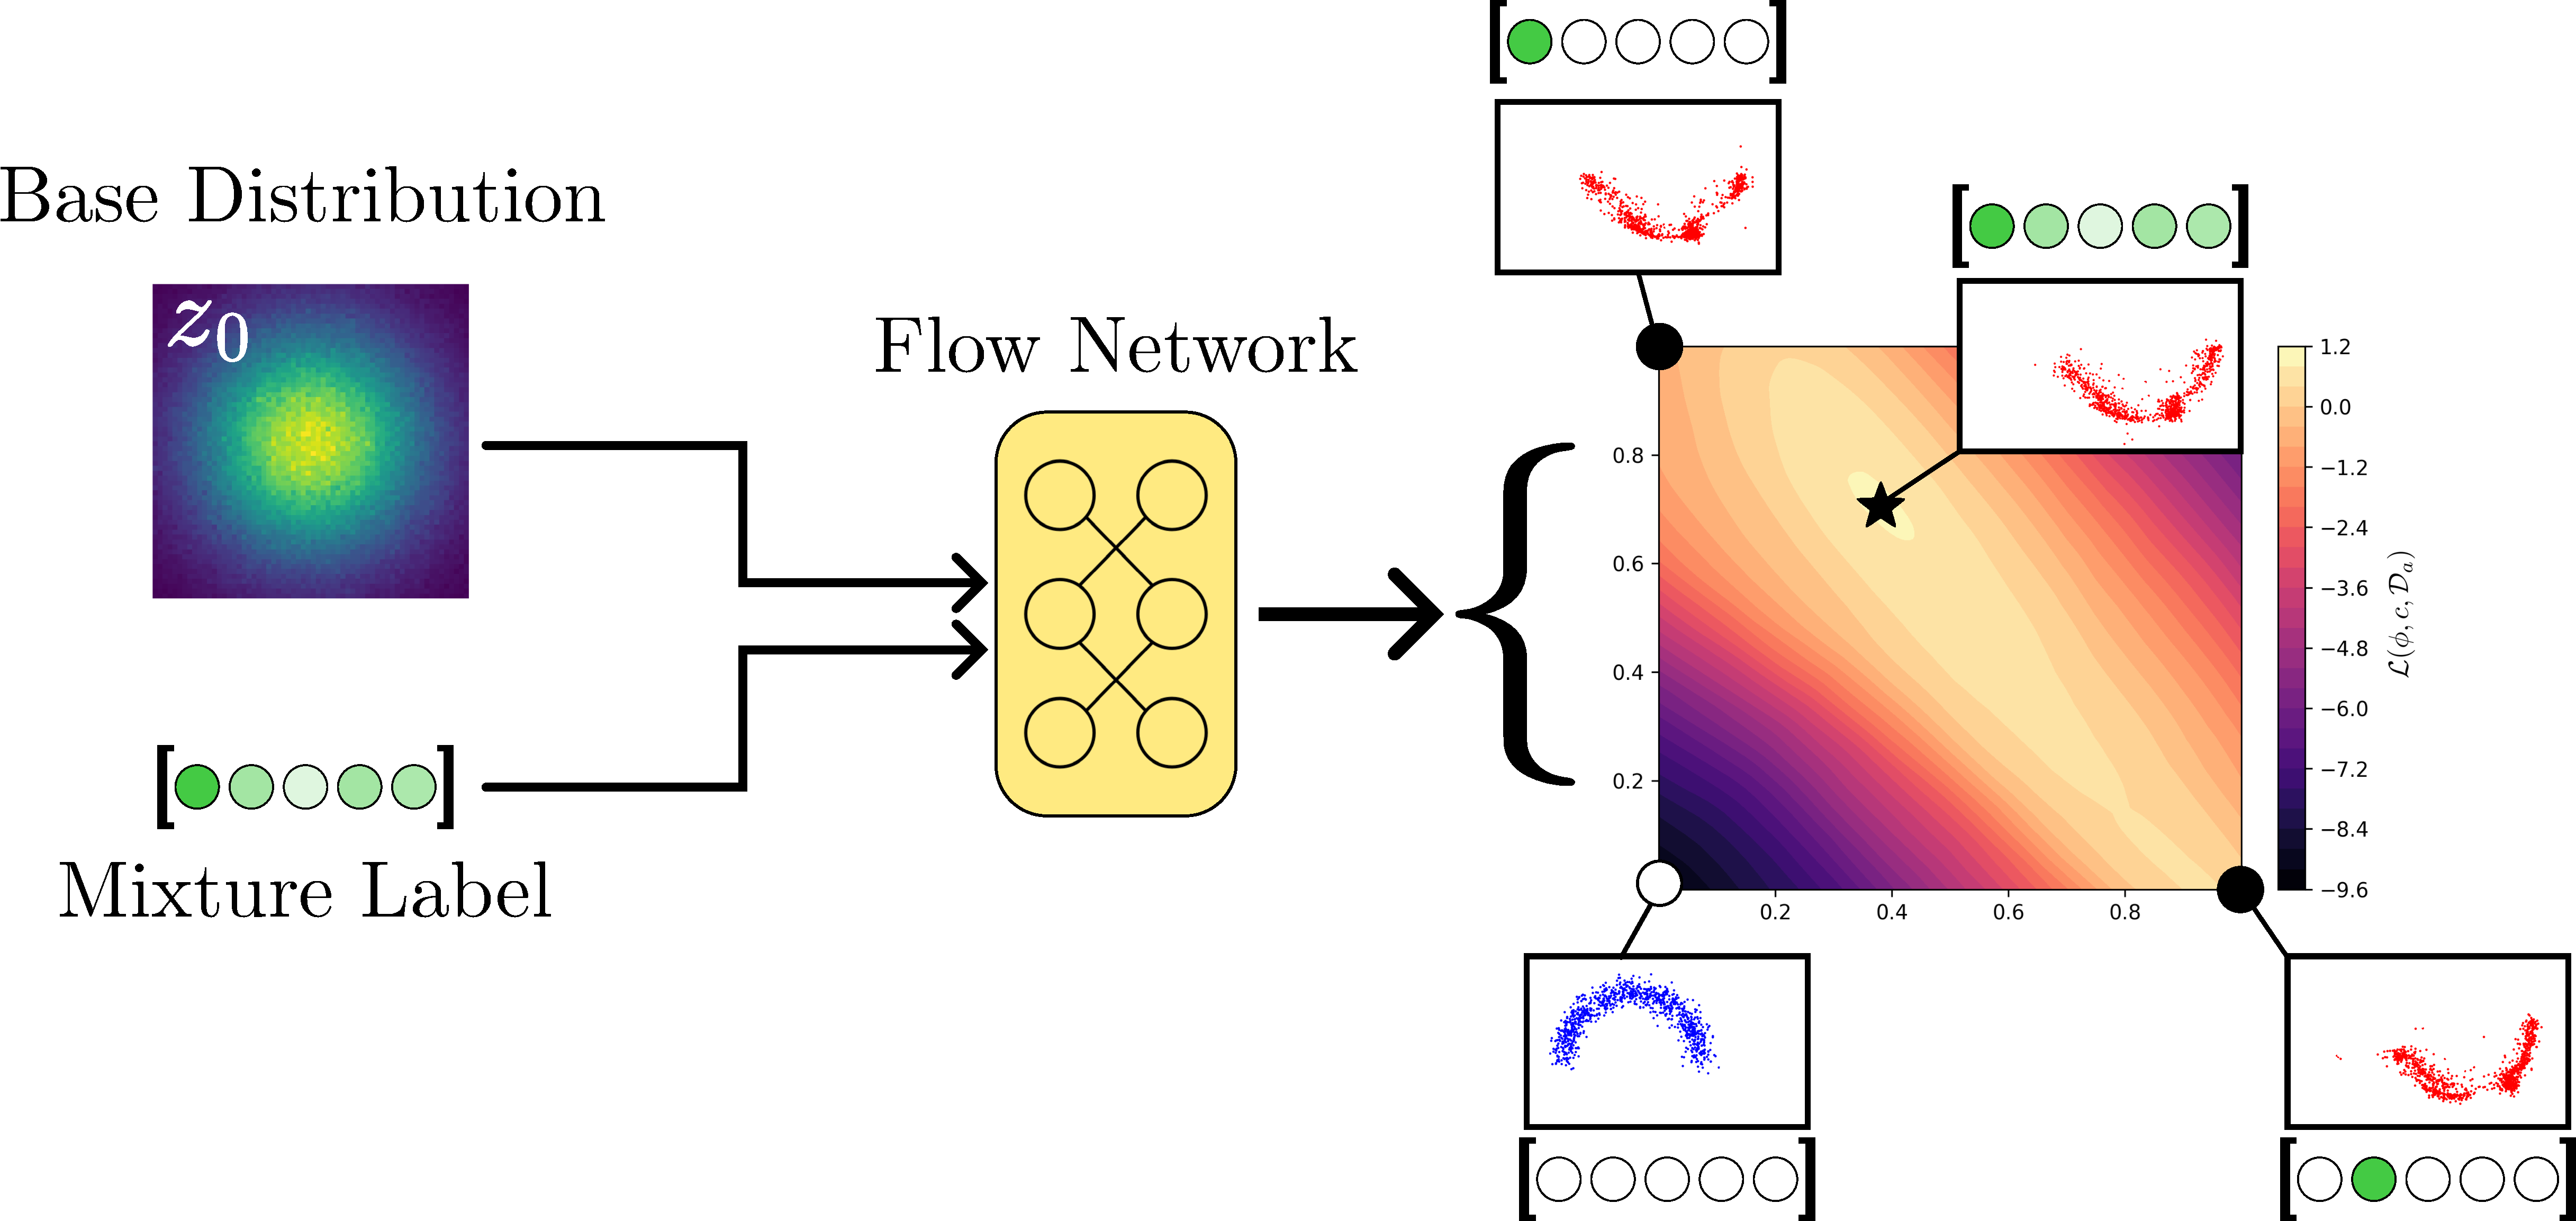
\includegraphics[width=\linewidth]{images/icml/architecture.pdf}
    \caption{
        \textbf{CalNF architecture}: A normalizing flow is trained on random subsets of the anomaly data and the full nominal dataset, using one-hot labels to identify different subsets ($\bullet$) and the zero vector to identify the nominal data ($\circ$). The model is calibrated by optimizing the label to find a posterior distribution that best explains the entire anomaly training dataset ($\bigstar$).}
    \label{ch:icml:fig:architecture}
\end{figure}

\ouralg{} begins by randomly sampling $K$ subsets of the anomaly data $\Df^1, \ldots, \Df^K$ and using a conditional flow $q_\phi(z; c)$ to learn a posterior for each, identifying the different subsets with one-hot labels $c_i = \mathbf{1}_i$:
\begin{align*}
    q_\phi(z; \mathbf{1}_i) & \approx p(z | \Df^i),\ i=1,\ldots,K \\
    q_\phi(z; \mathbf{0}_K) & \approx p(z | \Dn),
\end{align*}
where the zero label $c = \mathbf{0}_K$ is used to identify the nominal dataset. Once posteriors have been learned for each of these subsets, we calibrate the model by finding an optimal mixture of these posteriors to explain the full anomaly dataset; i.e. holding the model weights $\phi$ constant and finding the optimal label $c^*$ such that $q_\phi(z; c^*) \approx p(z | \Df)$.

This two-step process is illustrated in Fig.~\ref{ch:icml:fig:architecture}. On an intuitive level, our approach learns a family of anomaly posteriors parameterized by the low-dimensional label $c$, then optimizes in the lower-dimensional label space to find a good estimate of the overall anomaly posterior, as shown in Fig.~\ref{ch:icml:fig:architecture}.

It is important to note that \ouralg{} is agnostic to the specific architecture chosen for normalizing flow (e.g. the form of $f_\phi$). Our main contribution is the higher-level framework for training the model in the context of scarce anomaly data, which could in theory be used with any learned posterior representation.

\begin{algorithm}[H]
    \caption{Calibrated Normalizing Flows}
    \label{ch:icml:alg:calnf}
    \DontPrintSemicolon
    \KwInput{Nominal data $\Dn$, anomaly data $\Df$, step size $\gamma$, number of anomaly subsamples $K$}
    \KwOutput{Model parameters $\phi$ and calibrated label $c^*$}
    \For{$k = 1, \ldots, K$}
    {
        $\Df^k \gets \text{$\lfloor N_a/2 \rfloor$-element random subset of } \Df$\;
    }
    Initialize $\phi,\ c$\;
    \While{$\phi$ not converged}
    {
        Compute $L = L_a(\phi) + L_n(\phi) + L_{\text{cal}}(\phi, c)$\;
        Update model $\phi \gets \phi + \gamma \nabla_\phi L$\;
        Update calibration $c \gets c + \gamma \nabla_c L_{\text{cal}}(\phi, c)$\;
    }
\end{algorithm}

The \ouralg{} model, together with the optimized label, can be trained using Algorithm~\ref{ch:icml:alg:calnf}. This algorithm modifies the standard variational inference training process in two ways: by training on multiple random subsets of the anomaly data, and by interleaving model updates and label calibration.

First, we split the anomaly training data into $K$ random subsets with one-hot labels and train the model to learn the posterior for each subset. Each subset $\Df^i$ is created by independently drawing $\lfloor N_a/2 \rfloor$ samples from $\Df$ without replacement. We denote the ELBO on a given dataset $\mathcal{D}$ as
\begin{equation}
    \mathcal{L}\pn{\phi, c, \mathcal{D}} = \frac{1}{\abs{\mathcal{D}}} \sum_{(x, y) \in \mathcal{D}} \expectation_{z\sim q_{\phi}(z; c)}\left[ \log \frac{p(x, z; y)}{q_\phi(z; c)} \right].
\end{equation}

The model parameters are updated to maximize the sum of several ELBOs: for each anomaly subset (with one-hot labels), for the nominal dataset (with a zero label), and for the full anomaly dataset (with the calibrated label $c$):
\begin{align}
    L_{a}(\phi) =    & -\frac{1}{K} \sum_{i=1}^K \mathcal{L}\pn{\phi, \mathbf{1}_i, \Df^i}, \\
    L_{n}(\phi) =    & -\mathcal{L}\pn{\phi, \mathbf{0}_K, \Dn},                            \\
    L_{cal}(\phi, c) & = -\mathcal{L}(\phi, c, \Df)
\end{align}
This leads to the overall loss,
\begin{align}
    L(\phi, c) = & L_{a}(\phi) + L_{n}(\phi) + L_{cal}(\phi, c).
\end{align}

The mixture label $c$ is initialized at $[1/K, \ldots, 1/K]$ and updated to minimize $L_{cal}(\phi, c)$. In practice, we find that we can interleave optimization for $\phi$ and $c$.

\section{Experiments}\label{ch:icml:experiments}

\subsection{Benchmark problems}\label{ch:icml:examples}

This section briefly introduces the data-constrained anomaly diagnosis problems used in our experiments. More details on each problem is provided in the appendix, and we will open-source code and data for each upon publication. The first benchmark is newly developed to support our case study, but the second and third are previously-published benchmark problems~\cite{keipourALFADatasetUAV2021,dengOpenFWILargescaleMultistructural2022}.

\paragraph{Air traffic disruptions} We develop a stochastic queuing model of the Southwest Airlines network using actual flight arrival and departure data published by the US Bureau of Transportation Statistics~\cite{bureauoftransportationstatisticsTranStatsDepartmentTransportation}. This model tracks the movement of aircraft between airports in the network, accounting for randomness in travel times, runway use times, and air traffic control (ATC) delays, as well as runway congestion and varying aircraft reserves at each airport. We base our model off of that in~\cite{pyrgiotisModellingDelayPropagation2013}, with extensions to account for aircraft reserves. The latent variables represent travel times between airports, runway delays at each airport, and the number of aircraft stationed at each airport at the start of the day. The context includes the scheduled departures and arrivals for the day, and the observations include the actual departure and arrival time for each flight.

The nominal and anomaly datasets include data from December 1 through December 20 and December 21 through December 30 of 2022, respectively. For benchmarking, we consider only the four busiest airports in the Southwest network, but we consider larger sub-networks in our case study in Section~\ref{ch:icml:wn-case-study}. The four-airport sub-network has 24 latent variables. We train on $N_n = 9$ and $N_f = 4$ data points and evaluate on $4$ anomalous data points (each data point is a single day with between 88--102 flights).

\paragraph{Geophysical imaging} Seismic waveform inversion (SWI) is a well-known geophysics problem used as a benchmark for inference and physics-informed learning~\cite{gouveiaBayesianSeismicWaveform1998,dengOpenFWILargescaleMultistructural2022,zhangBayesianSpatialModelling2016}. SWI seeks to infer the properties of the Earth's subsurface using seismic measurements. A source emits a sound wave that travels through the Earth before being measured by several receivers. The wave is simulated by solving the elastic wave partial differential equation (PDE) numerically, with latent variables $z$ for the subsurface density profile, context $y$ for the source signal, and observations $x$ of the signal measured at each receiver~\cite{richardsonDeepwave2023}. The latent space has 100 dimensions. We train using $N_n = 100$ and $N_a = 4$ samples and evaluate on $500$ synthetic anomaly samples.

\paragraph{Aerial vehicle control} We also consider a failure detection benchmark for unmanned aerial vehicles (UAVs) using the ALFA dataset~\cite{keipourALFADatasetUAV2021}. This dataset includes real-world data from a UAV during normal flight and during a series of failures where various control surfaces are deactivated. In this case, $z$ parametrizes the nonlinear attitude dynamics, $y$ includes the current state and desired orientations, and $x$ is the next state. The latent space has 22 dimensions; we train on 10 nominal trajectories with $N_n = 2235$ data points and 1 anomalous trajectory with $N_a = 58$, and we evaluate on a second anomalous trajectory with $69$ data points (both the training and evaluation anomalies are rudder failures).

\paragraph{Other benchmarks} For completeness, we include results from the toy 2D problem in Fig.~\ref{ch:icml:fig:toy_example} ($N_n = 1000$, $N_f = 20$).

\subsection{Baselines and metrics}

Our main claim is that our \ouralg{} framework is an effective way to learn the posterior when a small number of anomaly data points are available. As a result, the most relevant comparisons are to methods for posterior learning with dataset bias, which typically involve regularizing the learned posterior. In particular, we compare against two baselines: a ``state-of-the-practice'' method regularizing the KL divergence~\cite{asimInvertibleGenerativeModels2020,higginsBetaVAELearningBasic2016} and a state-of-the-art method specific to normalizing flows that regularizes the Wasserstein distance $W_2$. This second method follows RNODE and related works by penalizing the squared norm of the vector field of a continuous normalizing flow~\cite{finlayHowTrainYour2020,onkenOTFlowFastAccurate2021}. We implement the KL-regularized method using neural spline flows~\cite{durkanNeuralSplineFlows2019} and label this method $\beta$-NSF. Since each of these baselines relies on a hyperparameter to determine the strength of the regularization ($\beta$ for KL regularization and $\lambda_K$ for RNODE), we provide results for a range of hyperparameters.

Since the relatively large amount of nominal data makes it easy to fit the nominal distribution, we compare primarily on the basis of the evidence lower bound $\mathcal{L}$ computed on held-out anomaly data. It is important to note that while our method requires less hyperparameter tuning than the other methods, it requires additional likelihood evaluations to fit the subsampled anomaly data. To quantify this trade-off, we report the training time for all methods. All metrics report the mean and standard deviation over four random seeds. When useful, we also provide visual comparisons of the posterior distributions learned using different methods.

We implement \ouralg{} using neural spline flows (NSF) as the underlying normalizing flow~\cite{durkanNeuralSplineFlows2019}. Since \ouralg{} is agnostic to the underlying flow architecture, we also tried masked autoregressive flows~\cite{huangNeuralAutoregressiveFlows2018}, which trained faster but had slightly worse performance, and continuous normalizing flows~\cite{chenNeuralOrdinaryDifferential2018}, which trained much more slowly.

We implement $\beta$-NSF using neural spline flows with a KL regularization penalty between the learned anomaly and nominal posteriors. We implement an RNODE-derived method that includes only the $W_2$ regularization term, not the Froebenius norm regularization term (which is used only to speed training and inference, not to regularize the learned posterior;~\cite{finlayHowTrainYour2020}).

All methods were implemented in Pytorch using the Zuko library for normalizing flows~\cite{ProbabilistsZuko2024}. The neural spline flows used 3 stacked transforms, and all flows used two hidden layers of 64 units each with ReLU activation (except for the continous flows on the 2D problem, which use two hidden layers of 128 units each). All flows were trained using the Adam optimizer with the learning rate $10^{-3}$ (except on the UAV problem, which used a learning rate of $10^{-2}$) and gradient clipping. \ouralg{} used $K=5$ on all problems. All methods were trained on a single Nvidia GeForce RTX 2080 Ti GPU, with 200, 500, 1000, and 300 epochs for the 2D, SWI, UAV, and ATC problems, respectively.

\subsection{Results \& discussion}

\begin{table}[htb]
    \caption{ELBO (nats/dim) on held-out anomaly data and training times (in minutes) on benchmark problems. 2D and SWI use synthetic data, so additional anomaly data were generated for the test set; in all other cases, half of the anomaly data was withheld for testing. Mean and standard deviation across four seeds are reported. Our method takes longer to train (requiring $K$ times as many likelihood evaluations) but meets or exceeds the state of the art without needing additional hyperparameter tuning. {}\textsuperscript{\textdagger}scaled by $\times 10^{-3}$}
    \label{ch:icml:tab:results}
    \begin{center}
        \begin{small}
            \begin{sc}
                \begin{tabular}{lcccc}
                    \toprule
                                                 & 2D                          & SWI                                              & UAV                        & ATC                                              \\ % & MNIST                \\
                                                 & nats/dim  $\uparrow$        & nats/dim\textsuperscript{\textdagger} $\uparrow$ & nats/dim  $\uparrow$       & nats/dim\textsuperscript{\textdagger} $\uparrow$ \\ % & nats/dim  $\uparrow$ \\
                    \midrule
                    $\beta$-NSF ($\beta = 0.01$) & $-3.22_{\pm 0.13}$          & $43.8_{\pm 0.61}$                                & $3.30_{\pm 0.83}$          & $-2.33_{\pm 0.05}$                               \\ % &                      \\
                    $\beta$-NSF ($\beta = 0.1$)  & $-2.03_{\pm 0.04}$          & $43.9_{\pm 0.79}$                                & $3.64_{\pm 1.27}$          & $-2.30_{\pm 0.05}$                               \\ % &                      \\
                    $\beta$-NSF ($\beta = 1.0$)  & $-1.04_{\pm 0.06}$          & $44.1_{\pm 0.84}$                                & $2.78_{\pm 1.71}$          & $-2.12_{\pm 0.09}$                               \\ % &                      \\
                    RNODE ($\lambda_K = 0.01$)   & $-4.58_{\pm 0.18}$          & $36.0_{\pm 3.14}$                                & $0.76_{\pm 2.31}$          & $-4.36_{\pm 1.02}$                               \\ % &                      \\
                    RNODE ($\lambda_K = 0.1$)    & $-2.95_{\pm 0.14}$          & $36.0_{\pm 3.13}$                                & $0.76_{\pm 2.28}$          & $-4.39_{\pm 1.08}$                               \\ % &                      \\
                    RNODE ($\lambda_K = 1.0$)    & $-1.67_{\pm 0.05}$          & $36.0_{\pm 3.06}$                                & $1.14_{\pm 2.50}$          & $-4.35_{\pm 1.04}$                               \\ % &                      \\
                    CalNF (ours)                 & $\mathbf{-0.90}_{\pm 0.10}$ & $\mathbf{46.3}_{\pm 0.18}$                       & $\mathbf{6.95}_{\pm 1.24}$ & $\mathbf{-2.01}_{\pm 0.10}$                      \\ % &                      \\
                    % CalNF w/o $c^*$              & $-0.96_{\pm 0.2}$           & $46.2_{\pm 0.4}$                                 & $\mathbf{7.86}_{\pm 1.0}$ & $-2.02_{\pm 0.1}$                                \\
                    % CalNF w/o $L_n$              & $-1.12_{\pm 0.2}$           & $46.1_{\pm 0.4}$                                 & $-9.22_{\pm 10}$          & $-2.03_{\pm 0.2}$                                \\
                    % CalNF w/o $\Df^i$            & $-1.03_{\pm 0.2}$           & $43.9_{\pm 2.8}$                                 & $-3.65_{\pm 11}$          & $-2.05_{\pm 0.1}$                                \\
                    \midrule
                                                 & Time $\downarrow$           & Time $\downarrow$                                & Time $\downarrow$          & Time $\downarrow$                                \\ % & Time $\downarrow$    \\
                    $\beta$-NSF ($\beta = 0.01$) & $\mathbf{0.43}_{\pm 0.02}$  & $33.5_{\pm 0.2}$                                 & $\mathbf{16.9} \pm 0.09$   & $\mathbf{81.6}_{\pm 9.2}$                        \\ % &                      \\
                    $\beta$-NSF ($\beta = 0.1$)  & $\mathbf{0.45}_{\pm 0.03}$  & $33.6_{\pm 0.2}$                                 & $\mathbf{17.0} \pm 0.08$   & $\mathbf{81.7}_{\pm 8.5}$                        \\ % &                      \\
                    $\beta$-NSF ($\beta = 1.0$)  & $\mathbf{0.45}_{\pm 0.03}$  & $33.6_{\pm 0.1}$                                 & $\mathbf{16.9} \pm 0.28$   & $\mathbf{81.4}_{\pm 8.7}$                        \\ % &                      \\
                    RNODE ($\lambda_K = 0.01$)   & $5.37_{\pm 0.17}$           & $\mathbf{25.1}_{\pm 0.5}$                        & $68.0 \pm 2.98$            & $\mathbf{82.0}_{\pm 8.4}$                        \\ % &                      \\
                    RNODE ($\lambda_K = 0.1$)    & $5.38_{\pm 0.19}$           & $\mathbf{25.1}_{\pm 0.7}$                        & $67.5 \pm 3.60$            & $\mathbf{82.2}_{\pm 7.6}$                        \\ % &                      \\
                    RNODE ($\lambda_K = 1.0$)    & $5.23_{\pm 0.06}$           & $\mathbf{24.9}_{\pm 0.7}$                        & $69.7 \pm 12.6$            & $\mathbf{81.8}_{\pm 8.7}$                        \\ % &                      \\
                    CalNF (ours)                 & $0.53_{\pm 0.02}$           & $80.1_{\pm 0.5}$                                 & $45.9 \pm 0.32$            & $148.8_{\pm 16.5}$                               \\ % &                      \\
                    \bottomrule
                \end{tabular}
            \end{sc}
        \end{small}
    \end{center}
    % \vskip -0.1in
\end{table}
\begin{table}[htb]
    \caption{ELBO (nats/dim) on held-out anomaly data for ablations of \ouralg{}. The first is our proposed method, the second fixes $c$, the third excludes the nominal data during training, and the fourth does not subsample the anomaly data. {}\textsuperscript{\textdagger}scaled by $\times 10^{-3}$}
    \label{ch:icml:tab:ablation}
    \vspace{-1em}
    \begin{center}
        \begin{small}
            \begin{sc}
                \begin{tabular}{lcccc}
                    \toprule
                                & 2D                         & SWI\textsuperscript{\textdagger} & UAV                       & ATC\textsuperscript{\textdagger} \\
                    \midrule
                    CalNF       & $\mathbf{-0.90}_{\pm 0.1}$ & $\mathbf{46.3}_{\pm 0.2}$        & $6.95_{\pm 1.2}$          & $\mathbf{-2.01}_{\pm 0.1}$       \\
                    w/o $c^*$   & $-0.96_{\pm 0.2}$          & $46.2_{\pm 0.4}$                 & $\mathbf{7.86}_{\pm 1.0}$ & $-2.02_{\pm 0.1}$                \\
                    w/o $L_n$   & $-1.12_{\pm 0.2}$          & $46.1_{\pm 0.4}$                 & $-9.22_{\pm 10}$          & $-2.03_{\pm 0.2}$                \\
                    w/o $\Df^i$ & $-1.03_{\pm 0.2}$          & $43.9_{\pm 2.8}$                 & $-3.65_{\pm 11}$          & $-2.05_{\pm 0.1}$                \\
                    \bottomrule
                \end{tabular}
            \end{sc}
        \end{small}
    \end{center}
    % \vskip -0.1in
\end{table}
\begin{figure}[tb]
    \centering
    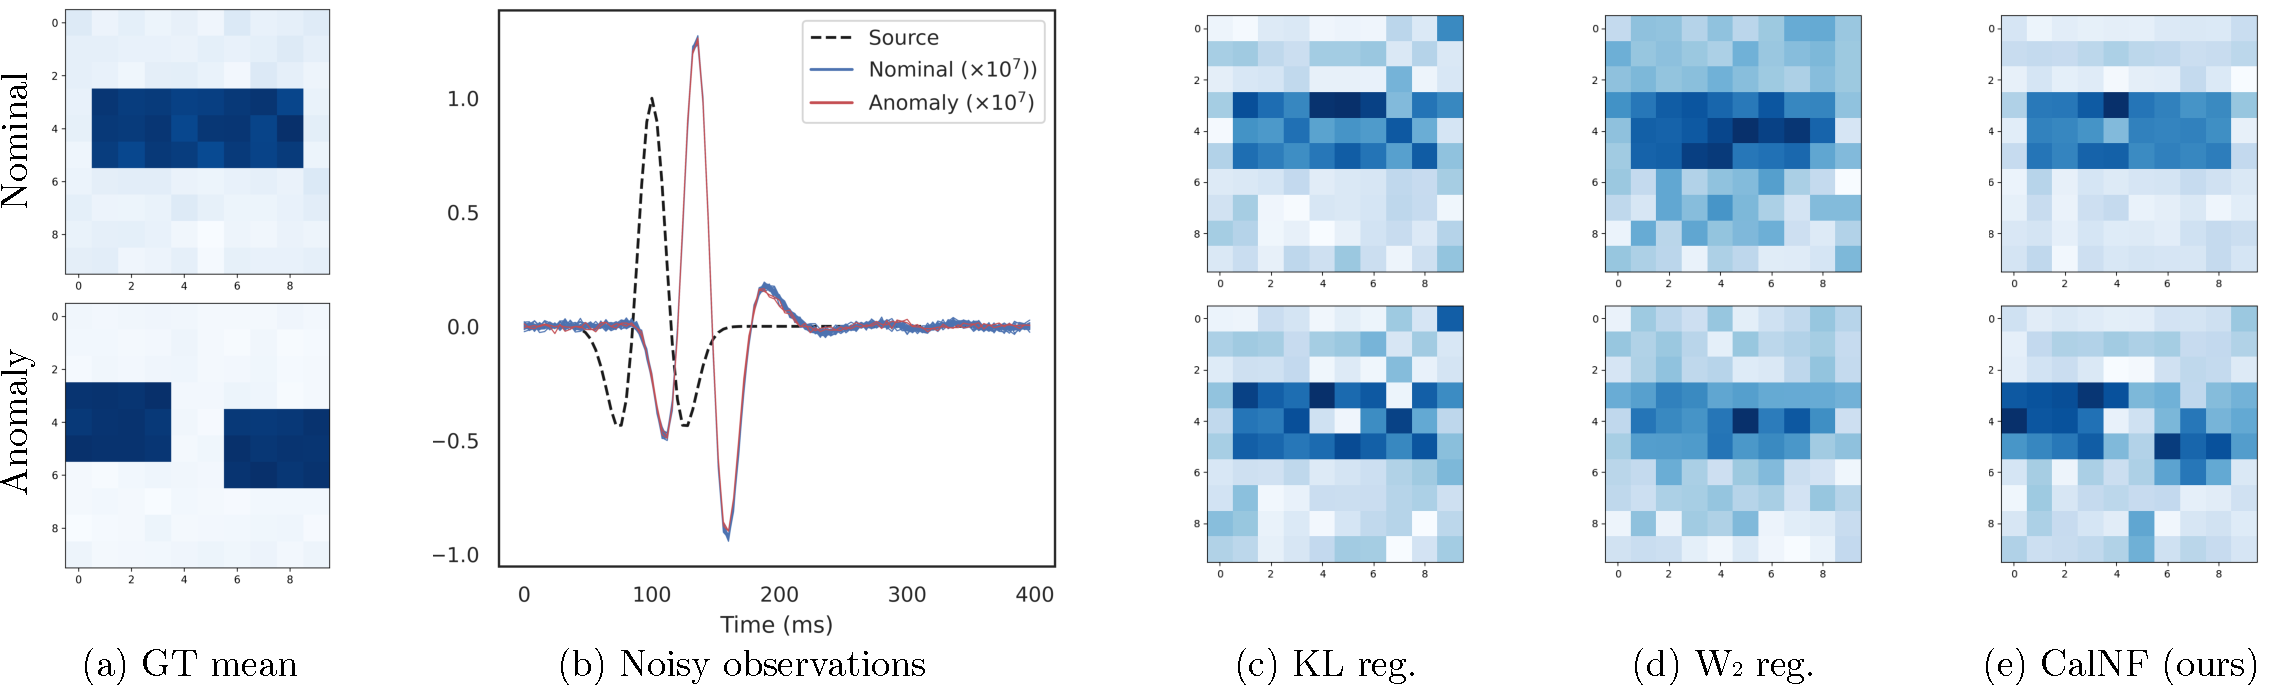
\includegraphics[width=\linewidth]{images/icml/swi_results/swi_summary.pdf}
    \caption{\textbf{Seismic waveform inversion.} (a) The ground truth nominal and anomalous density profiles. (b) The waveforms observed in each case. (c-e) The posteriors fit using KL regularization, $W_2$ regularization, and our \ouralg{} method. Ours is the only method to correctly infer the shape of the anomaly density profile.}
    \label{ch:icml:fig:swi_results}
\end{figure}

Our main empirical results are shown in Table~\ref{ch:icml:tab:results}. We find that our method achieves better performance on held-out anomaly data than baselines on all problems; moreover, our method does not require manual hyperparameter tuning ($K=5$ was sufficient for all problems). \ouralg{}'s improved performance comes at the cost of increased training time, requiring $K$ additional likelihood evaluations per step; this difference is most significant on the SWI and ATC problems, where evaluating the likelihood is particularly expensive. On problems where the likelihood is easy to evaluate, the RNODE-derived methods are slowest to train due to their use of neural ODEs.

To understand the difference in performance, Fig.~\ref{ch:icml:fig:swi_results} compares the learned anomaly posteriors on the SWI example, which lend themselves to easy visualization. \ref{ch:icml:fig:swi_results}a shows the ground truth subsurface profiles, and \ref{ch:icml:fig:swi_results}b shows the noisy observations.
%
We see that the two regularization-based methods are partially successful: the KL-regularized method (\ref{ch:icml:fig:swi_results}c) partially infers the break in the anomaly subsurface profile, and while the $W_2$-regularized method (\ref{ch:icml:fig:swi_results}d) does not infer the break, it does infer the increased uncertainty in the anomaly case. However, only our method (\ref{ch:icml:fig:swi_results}e) is able to correctly infer the shape of the anomaly profile. This suggests that our method is able to appropriately balance the information gained from the nominal distribution with the limited number of anomaly data points.

We also provide the results of an ablation study in Table~\ref{ch:icml:tab:ablation}, comparing the ELBO achieved when we omit the calibration step (using a constant $c$), omit the nominal data, and remove the subsampling step. These results indicate that most of the performance improvement from \ouralg{} is due to training on random subsamples of the anomaly data. We observe that in cases with plentiful nominal data (like the UAV problem), including the $L_n$ term also substantially boosts performance. We find that the benefit of optimizing $c$ is relatively minor compared to the other components, but this step can be included for little additional computational cost, re-using the likelihood evaluation and backward pass from the main model update.

\section{Post-mortem analysis of the 2022 Southwest Airlines scheduling crisis}\label{ch:icml:wn-case-study}

In this section, we apply our method to a post-mortem analysis of the 2022 Southwest Airlines scheduling crisis. In the period between December 21\textsuperscript{st} and December 30\textsuperscript{th}, 2022, a series of cascading delays and cancellations severely disrupted the Southwest network, starting in Denver and spreading across the United States. The disruption occurred in roughly two stages, as shown in Figs.~\ref{ch:icml:fig:wn_cancellations:timeline} and~\ref{ch:icml:fig:wn_cancellations:cancellations}. In the first stage, from 12/21 to 12/24, weather and operational difficulties caused cancellations to increase from a $< 5\%$ baseline to over $50\%$ of scheduled flights. In the second phase, after trying and failing to recover normal operations, Southwest flight dispatchers started preemptively cancelling flights and ferrying crew between airports to reset the network, cancelling up to $77\%$ of scheduled flights between 12/25 and 12/29 before returning to near-normal operations on 12/30. Southwest ultimately cancelled more than 16,000 flights, affecting more than 2 million passengers, and the airline later paid a \$140 million penalty imposed by the US Department of Transportation ($28\%$ of its 2023 net income;~\cite{roseSouthwestWillPay2023}) in addition to lost revenue.

\begin{figure}[tb]
    \centering
    \begin{subfigure}[t]{0.45\linewidth}
        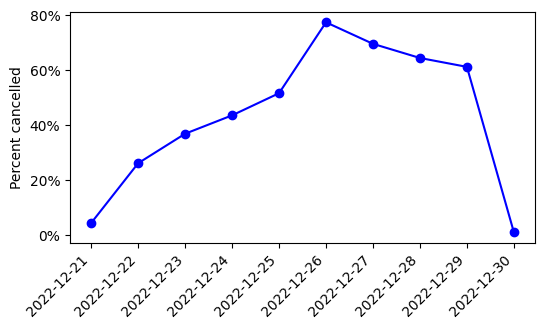
\includegraphics[width=\linewidth]{images/icml/wn/wn_cancellations.png}
        \caption{Timeline of cancellations during the 2022 Southwest Airlines scheduling crisis.}
        \label{ch:icml:fig:wn_cancellations:timeline}
    \end{subfigure}
    \begin{subfigure}[t]{0.45\linewidth}
        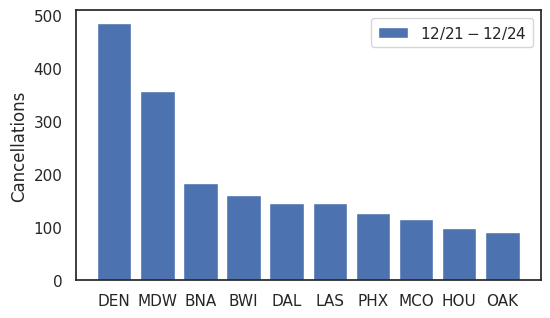
\includegraphics[width=\linewidth]{images/icml/wn/wn_cancellations_by_origin.png}
        \caption{Cancellations at the 10 busiest airports in Southwest's network during the first four days of the disruption.}
        \label{ch:icml:fig:wn_cancellations:cancellations}
    \end{subfigure}
    % \label{ch:icml:fig:wn_cancellations}
\end{figure}

This incident has been the subject of extensive investigation, with a report from Southwest Airlines~\cite{southwestairlinesFinalSummaryAction2023}, testimony before the US Senate from the Southwest Airlines Pilots Association (SWAPA;~\cite{MurrayTestimony}), and press coverage~\cite{roseSouthwestWillPay2023,cramerWhatCausedChaos2022}. These sources propose a number of hypotheses on the root cause of the 2022 incident. While there is broad agreement that winter weather was a major factor, sources differ on the role of other factors; e.g. the SWAPA report emphasizes poor crew management, while press coverage emphasizes the point-to-point nature of the Southwest network.

Given this context, we have two goals for our case study. First, we are interested in identifying changes in the network state that coincided with the disruption, and how those disrupted parameters compare to the nominal state of the network. Second, we aim to produce a generative model of the nominal and disrupted network conditions to act as a tool for network design and analysis, so that future operational, scheduling, and recovery policies might be proactively stress-tested.

\subsection{Implementation}

Due to the difficulty of modeling the decision-making process of the Southwest flight dispatchers during the second half of the disruption, we focus on the first four days of the scheduling crisis, prior to the wave of cancellations aimed at resetting the network. We conduct our analysis at multiple levels of spatial resolution, looking at both the top-4 and top-10 subnetworks that include only flights between the 4 and 10 busiest airports in the Southwest network, respectively.

We modify the \ouralg{} framework slightly for this use case; instead of randomly subsampling the anomaly data (one data point for each of the first four days of the crisis), we use each day of the crisis as a separate subsample $\Df^i$. This allows us to simultaneously fit a posterior for the overall disruption (using the calibrated label $c^*$) and for each individual day of the disruption, respecting the time-varying nature of this problem.

The input to our air traffic model is a list of scheduled flights, each specifying an origin and destination airport and a scheduled departure and arrival time. The latent state $z$ includes the mean travel time between each origin/destination pair, the mean service time at each airport (which affects both arriving and departing aircraft and models taxi, deicing, and ATC delays), the mean turnaround time at each airport (the minimum time that must elapse before an arriving aircraft may depart), the baseline cancellation rate at each airport, and the initial number of aircraft at each airport.

The model steps through the scheduled flights in 15 minute increments. In each increment, it checks for the flights that are scheduled to depart from each airport. Each of these flights receives a certain probability of cancellation given by
\begin{equation}
    P(\text{cancelled}) = 1 - (1 - p_c) \sigma\pn{10 \frac{\text{\# available aircraft}}{\text{\# departing flights in this block}}}
\end{equation}
where $p_c$ is the baseline cancellation rate for the origin airport and $\sigma$ is the sigmoid function, so the probability of cancellation is $p_c$ when there are more available aircraft than scheduled departures and approaches $1$ as the number of available aircraft decreases. Cancellations are sampled from a relaxed Bernoulli distribution with this cancellation probability and a straight-through gradient estimator. If a flight is cancelled, it is marked as such and the observation for that flight will just be \texttt{cancelled} and will not include actual departure and arrival times. If the flight is not cancelled, then it is moved to the runway queue if there are enough aircraft available; otherwise, it is delayed until the next time block.

Both departing and arriving flights are served using a single M/M/1 queue for each airport, with service times drawn from an exponential distribution with the mean specified according to each airport's mean service time. Once airborne, departing flights are assigned a random flight time from a Gaussian with mean given by the mean travel time for each route and fixed variance. Once this travel time has elapsed, they enter the runway queue at the destination airport. Once an aircraft has landed, it does not become available to serve new flights until the minimum turnaround time has elapsed (which is sampled from a Gaussian with mean given by the mean turnaround time for each airport). Observations for non-cancelled flights include the simulated arrival and departure times, plus some fixed-variance Gaussian noise.

For reference, Table~\ref{ch:icml:tab:airport_codes} includes a key of relevant three-letter airport codes.

\begin{table}[htb]
    \caption{International Air Transport Association (IATA) codes and full names of the ten busiest airports in the Southwest network.}
    \label{ch:icml:tab:airport_codes}
    \begin{center}
        \begin{small}
            \begin{tabular}{cl}
                \toprule
                DEN & Denver International Airport                                 \\
                DAL & Dallas Love Field Airport                                    \\
                MDW & Chicago Midway International Airport                         \\
                PHX & Phoenix Sky Harbor International Airport                     \\
                HOU & William P. Hobby Airport                                     \\
                LAS & McCarran International Airport                               \\
                MCO & Orlando International Airport                                \\
                BNA & Nashville International Airport                              \\
                BWI & Baltimore/Washington International Thurgood Marshall Airport \\
                OAK & Oakland International Airport                                \\
                \bottomrule
            \end{tabular}
        \end{small}
    \end{center}
    % \vskip -0.1in
\end{table}

\subsection{Results}

\paragraph{Localized delays due to winter weather.} Our first observation confirms a common explanation for the disruption: that localized delays at airports across the US coincided with winter weather. For example, Fig.~\ref{ch:icml:fig:wn_service_times} shows \ouralg{}'s posterior estimates of nominal and disrupted service times, which include taxiing, deicing, and ATC delays, at the four busiest airports. Of these four, DEN, MDW, and DAL, which saw severe cold temperatures, experienced a 50\% increase in average service time, while there was no corresponding increase at LAS, which did not experience severe weather.
%
This result agrees with press and official accounts that identify winter weather and a lack of deicing equipment at critical airports like DEN as a contributing factor~\cite{southwestairlinesFinalSummaryAction2023,cramerWhatCausedChaos2022}. However, the more important question is how these localized service delays cascaded into the nationwide disruption.

\begin{figure}[t]
    \centering
    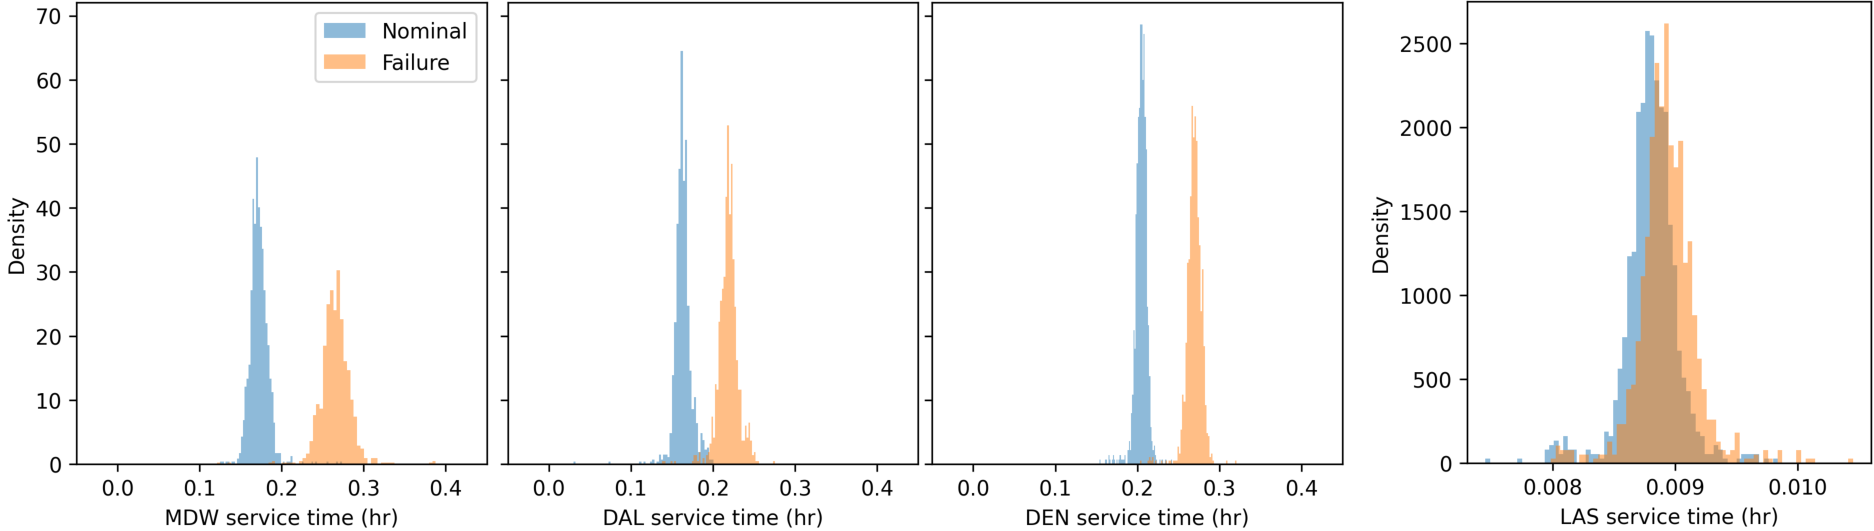
\includegraphics[width=\linewidth]{images/icml/wn/wn_top4_service_times.pdf}
    \caption{The posterior distribution indicates that service times (including taxiing, de-icing, and ATC delays) increased at DEN, MDW, and DAL, which were hit by a winter storm, but were unchanged at LAS, which did not see severe weather.}
    \label{ch:icml:fig:wn_service_times}
\end{figure}

\paragraph{Cascading failures due to aircraft flow interruption.}
%
Our main finding comes from modeling the movement of aircraft within the Southwest network. The number of aircraft that start the day at each airport provides an important measure of robustness, since if there are insufficient aircraft to meet demand, then departing flights must be delayed or canceled.\footnote{The same logic holds for the crew distribution. Our model assumes that crews and aircraft move together, but a separate crew model with duty time limits would be an important extension.} A lack of aircraft can also cause cancellations to cascade through the network if down-stream airports are deprived of the aircraft needed to serve scheduled departures. Despite its importance, aircraft distribution is not directly observable from public data, and so it must be inferred.

\begin{figure}[htb]
    \centering
    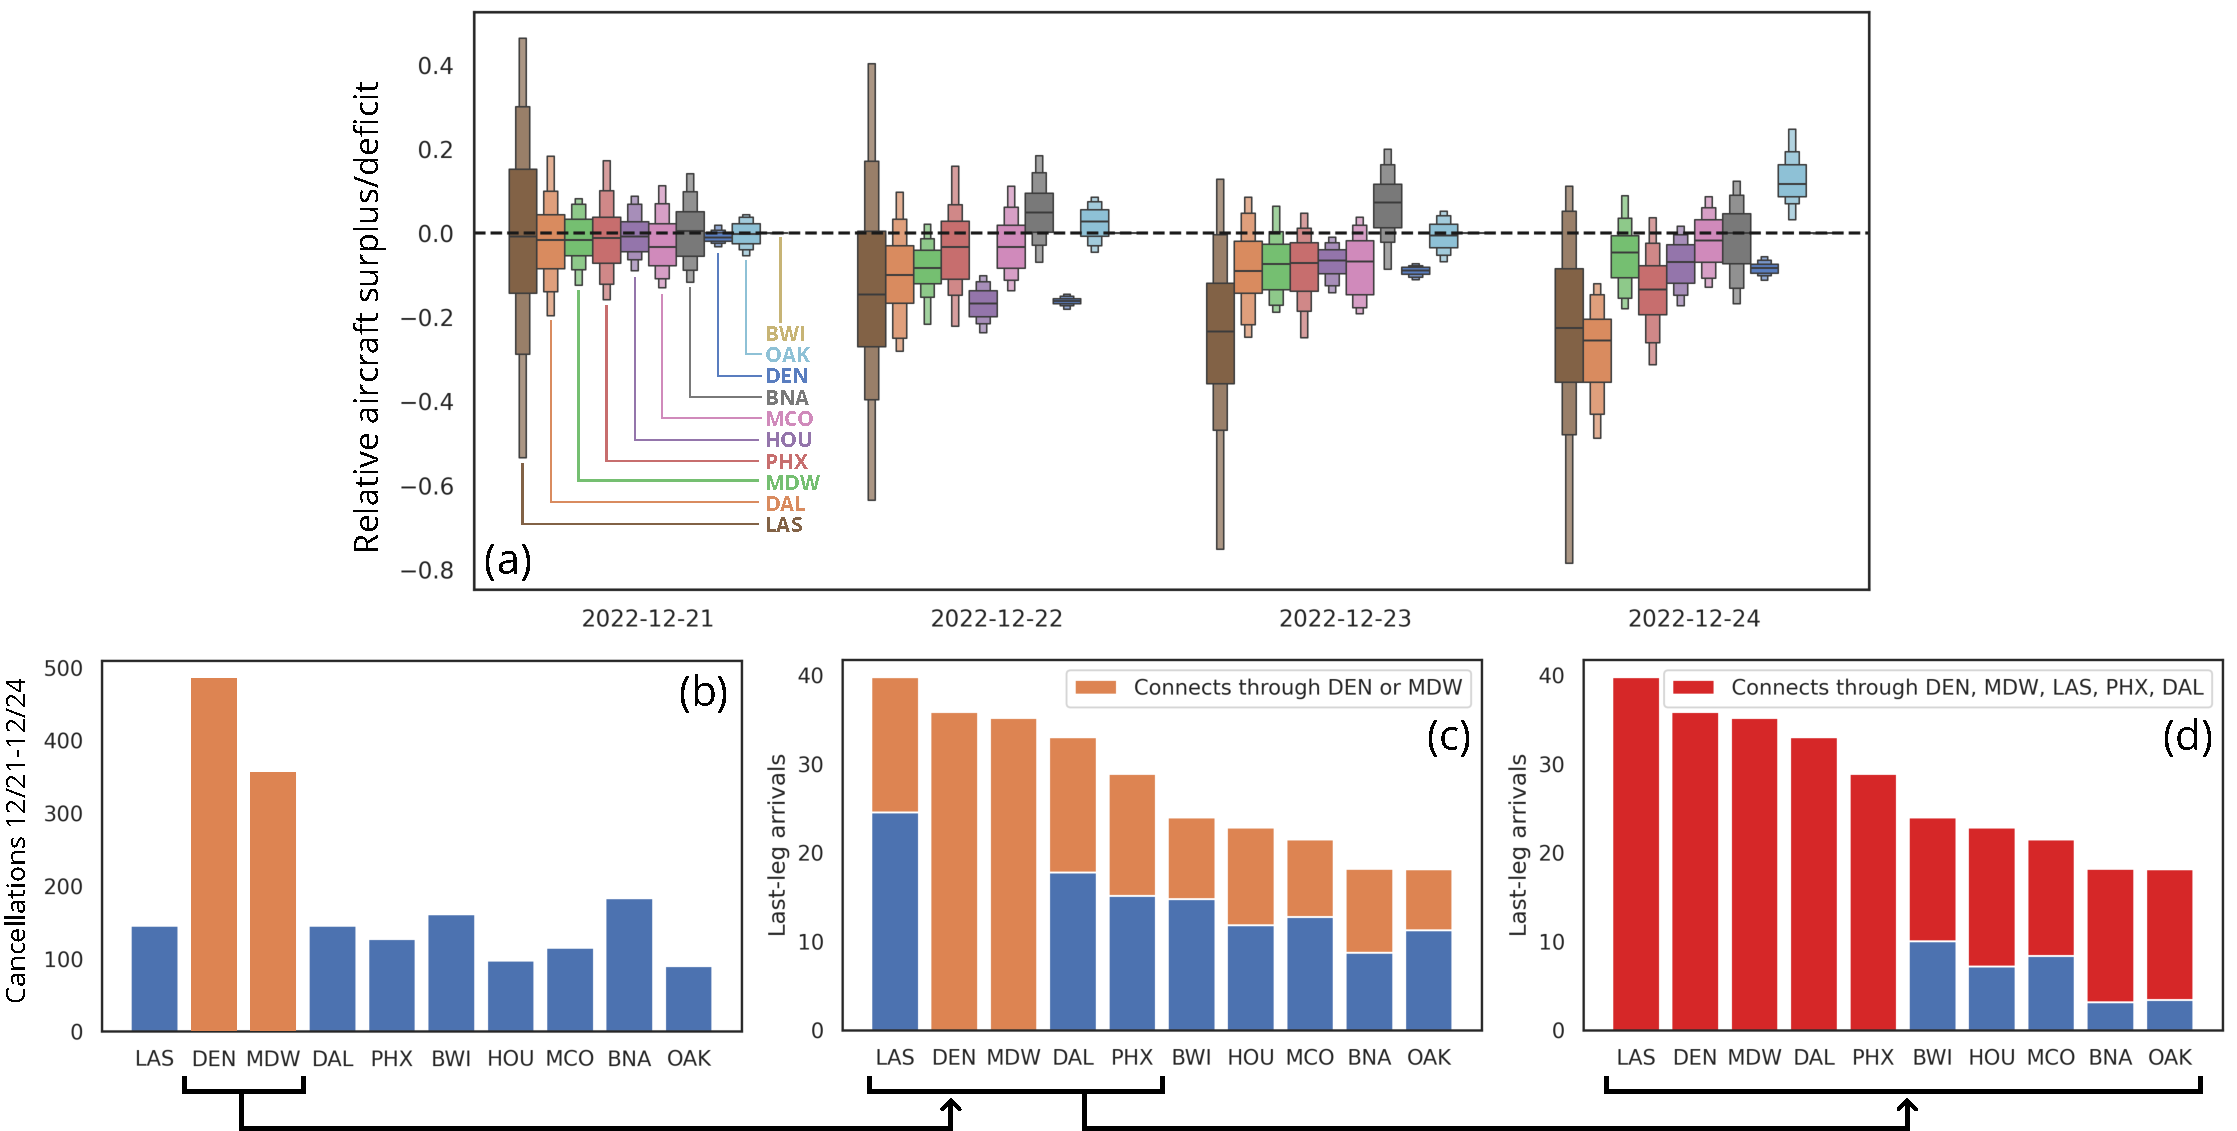
\includegraphics[width=\linewidth]{images/icml/wn/wn_reserves.pdf}
    \caption{(a) Posterior estimates (inferred using our method) of the distribution of Southwest aircraft at the start of the first four days of the disruption, normalized by the number of scheduled departures at each airport; positive/negative indicates more/fewer aircraft than in the nominal case, respectively. We see that LAS, DAL, and PHX accumulate a large aircraft deficit over the course of the disruption.
        %
        (b) Cancellations during the first four days of the disruption were concentrated in DEN and MDW.
        %
        (c) During normal operations, LAS, DAL, and PHX (together with DEN and MDW) host the five largest overnight aircraft reserves in the network (i.e. the largest number of arrivals on the last leg of each aircraft's daily sequence). Cancellations at DEN and MDW may have cascaded to create the deficits at LAS/DAL/PHX that we observe using our method.
        %
        (d) The large majority of normally-scheduled flights in the network connect through either DEN/MDW or LAS/DAL/PHX. Our analysis with \ouralg{} suggests that the overnight aircraft reserves at LAS, PHX, and DAL played a key role in propagating weather-related disruptions at DEN and MDW to the rest of the network.
    }
    \label{ch:icml:fig:wn_reserves}
\end{figure}

Fig.~\ref{ch:icml:fig:wn_reserves} shows our results from inferring the distribution of aircraft in the top-10 network. We use \ouralg{} to learn the posterior distribution for each of the first four days of the disruption, then plot this inferred aircraft distribution over time. Fig.~\ref{ch:icml:fig:wn_reserves}a shows that there was no detectable deviation from the nominal aircraft distribution on the first day of the disruption, but we see a steadily increasing deficit at LAS, DAL, and PHX over the following three days. The fact that the aircraft deficit at these airports continued to worsen may have been a factor in Southwest's decision to ``hard reset'' the network by ferrying empty planes between airports.

Figs.~\ref{ch:icml:fig:wn_reserves}(b-d) show how these accumulating deficits connect localized weather-related disruptions to system-wide failure. Fig.~\ref{ch:icml:fig:wn_reserves}(b) shows how cancellations during the first four days were concentrated at DEN and MDW; these cancellations likely contributed to decreased aicraft reserves at LAS, PHX, and DAL, which receive nearly 50\% of their last-leg flights\footnote{Aircraft arriving on the last leg of their flight sequence for the day, which remain at the airport overnight.} from either DEN or MDW, per Fig.~\ref{ch:icml:fig:wn_reserves}(c). LAS, PHX, and DAL, together with DEN and MDW, host the five largest overnight aircraft reserves in the network, and the rest of the Southwest network receives the vast majority of their incoming flights from routes visiting these airports, as shown in Fig.~\ref{ch:icml:fig:wn_reserves}(d). Even though LAS and PHX did not see the same severe winter weather as DEN and MDW (DAL did experience freezing temperatures), our analysis suggests that LAS, PHX, and DAL may have played a key role in allowing the disruption to spread throughout the Southwest network. Our results indicate that trends in overnight aircraft reserves at these airports may be a valuable warning sign for detecting future disruptions.

\paragraph{Generative modeling} Once we have learned the nominal and disruption posteriors for the Southwest network, we can use these as generative models for stress-testing proposed modifications to the Southwest network or scheduling system. In future work, we hope to explore how these generative models can be used to design more resilient schedule recovery algorithms.

\section{Summary}\label{ch:icml:conclusion}

In this chapter, we propose a novel algorithm for data-constrained posterior inference, which uses a subsampling and calibration strategy to avoid overfitting to scarce data. We apply our algorithm to anomaly diagnosis problems, achieving competitive performance on challenging inverse problem benchmarks with both simulated and real data. We also apply our algorithm to a real-world anomaly diagnosis problem, providing new insight into the factors behind the 2022 Southwest Airlines scheduling crisis.

\paragraph{Limitations \& future work} There are two major limitations of our work, which indicate directions for future research. First, it has been reported that normalizing flows struggle on out-of-distribution detection tasks, since they can assign high likelihoods to out-of-distribution samples~\cite{kirichenkoWhyNormalizingFlows2020}. Since our method relies heavily on normalizing flows, more work is needed before our method can be used to detect previously-unseen anomalies, building on existing out-of-distribution detection techniques.

Second, our method does not provide any estimate of the risk associated with that anomaly (i.e. how likely was it?). Estimating the risk of failure is challenging due to the size of the dataset, but we hope that future work will close this gap, potentially through the application of large deviation theory~\cite{demboLargeDeviationsTechniques2010}, allowing us to not only explain observed anomalies but also estimate their probability of occurrence.

In addition, we hope to further explore how the nominal and anomaly posterior distributions can be used as generative models for developing improved control algorithms; for example, using the learned model of UAV failures to optimize a flight controller, or using the learned model of the Southwest Airlines disruption to design improved scheduling and recovery algorithms.